\section{A* decoder for Shift-Reduce Parsing}
A* search is a very well-known algorithm which belongs to the best-first algorithm. The best-first algorithm uses an agenda to store all the processed points in the searching process. In each step, the most promising point will be used to extend until we reach the final point. 

However, unlike the regular best first algorithm which uses only the path cost $g(x)$ of each point $x$ in agenda to calculate the best point, A* algorithm also uses an heuristic $h(x)$ which is an admissible heuristic of the path from $x$ to the final point. It means that each point $x$ in A* algorithm will have the score calculated by:

\begin{equation}
	score(x) = g(x)+h(x)
\end{equation}

A* algorithm can guarantee to find the goal with smallest path cost in a shorter time than regular best-first search. To make sure that A* algorithm is efficient, $h(x)$ should satisfy two characters:
\begin{itemize}
	\item admissible: the heuristic must be greater or equal than the real highest cost we have to take in order to get to the final point: $h(x) \geq h_{real}(x)$
	\item consistency: $h(x) \leq d(x,y)+h(y)$, for every ($x,y$) where $y$ is next to $x$, $d(x,y)$ is the cost from $x$ to $y$. This is an additional condition.
\end{itemize}
Therefore, it is plain to see that $h(x)$ is the key of A* algorithm's efficiency.

\subsection{Best first decoder}
In order to utilize A* heuristic, we firstly built our best first decoder which is similar the one in \cite{ref:2014David} but for constituent parsing. Let us denote that $BFS(x)$ is the candidate final state returned by the best first decoder. The best first decoder can be described as follows:
\begin{itemize}
	\item Set up an agenda adding the initial state.
	\item In each step, popping out the best candidate in agenda and extend it by using the shift-reduce actions. After that, put the newly constructed states back into agenda.
	\item Looping until the popped candidate from agenda is the final state.
\end{itemize}

In best first decoder, the model score of each state $s$ is the cost path, the model score of each shift-reduce actions $a_i$ is the transition cost between each state. Let us recall that the model score of state $s$ is the sum of model score of all its shift-reduce actions $a_i$ as in (4). The model score of $a_i$ is calculated as in equation (5). If we use A* decoder, $score(s)$ will be calculated by $g(s)+h(s)$, where $h(s)$ is the heuristic which will be discussed in the next section. The training process of shift-reduce parsing with best first decoder is illustrated in table \ref{best first perceptron}.

\begin{equation}
	score(s) = g(s) = \sum_{i = 0}^{N} score(a_i)
\end{equation}

\begin{equation}
	score(a_i) = \Phi(a_i).\vec{w}
\end{equation}

\begin{table*}[t]
	\begin{center}
		\caption{\label{best first perceptron} Averaged perceptron algorithm with best first search decoder.}
		\begin{tabular}{|l|l|}
			\hline
			\bf Inputs & Training examples ($x_i,y_i$) \\
			\bf Initialization & $\vec{w}$ = 0 \\
			\bf Output & averaged weights $\vec{w}$ \\
			\hline
			\bf Algorithm 	& For $t = 1 ...T, i = 1 ...n$ \\
			& --- Calculate $F(x_i) = BFS(x_i)$ \\
			& --- If $(F(x_i) \neq y_i)$ then $\vec{w} = \vec{w} + \Phi(y_i) - \Phi(z_i)$ \\
			\hline							
		\end{tabular}
	\end{center}
\end{table*}

The only remain bottle-neck is that the negative score problem happened in the shift-reduce parsing process. In best-first search algorithm, the transition of each shift-reduce actions must be positive. However, due to the learning strategy of averaged perceptron, there still exist a negative value in the weights vector $\vec{w}$, and this may lead to negative score problem. Concerning about this problem, we solved this by adding a certain offset value to the transition score of each actions to keep it positive. Because the number of shift-reduce actions is always $2n$ (section 2.3) in our system, the rank of final states is still the same as before. So it will be able to apply this method.

\begin{table*}
	\begin{center}
		\caption{\label{first experiment} The experiment on the development set.}
		\begin{tabular}{|p{2cm}|p{3cm}|p{3cm}|p{3cm}|p{3cm}|}
			\hline 
			System & F-score on BF & parsing speed on BF & F-score on SF & parsing speed on SF \\ \hline
			beam search decoder with $beam = 16$ & 89.07\% & 25 sentences/s & 88.72\% & 30 sentences/s \\ \hline
			beam search decoder with $beam = 32$ & 89.87\% & 10 sentences/s & 89.33\% & 13 sentences/s \\ \hline	
			beam search decoder with $beam = 64$ & 90.3\% & 3.4 sentences/s & 90.15\% & 4.5 sentences/s \\ \hline
			beam search decoder with $beam = 128$ & & & & \\ \hline
			$A*$ decoder & N/A & N/A & 90.7\% & 1.2 sentences/s \\
			\hline
		\end{tabular}
	\end{center}
\end{table*}


\subsection{Grammar projection}
\textit{Grammar projection} is an interesting idea published in \cite{ref:2003Dan1} and this may be the first research on A* parsing in our knowledge. In this method, they have projected the original grammar rules to a simpler grammar rules. Each projected production rule always have the PCFG probability that is the maximum value of all the original production rules projecting to it. With this conversion, the outside PCFG score of the parse tree constructed by this projected grammar is always greater or equal to the real outside PCFG score and it can be an heuristic for A* search.

In our system, we design our own grammar projection based on the filter projection from \cite{ref:2003Dan1} with some modification which is suitable with shift-reduce parsing:
\begin{itemize}
	\item project all the complete constituent tags such as [NP, VP, ADJP...] into one single label called [XTAG].
	\item keeping all the incomplete constituent tags such as [NP*, AP*, ADJP*] and the PoS tag as before.
\end{itemize}

Corresponding to this projection, the features will also be projected in our system. The projected features will have the weight equaling the maximum value of all features which project it. For example, there are shift features whose types are $s_0.fw$+$s_0.c$ with values: ([google+VP]; [google+NP]; [google+AP]) with the weights (14.65; 5.67; 8.2), respectively. They will be projected into one value: [google+XTAG] with the weight equaling to 14.65.

In our A* decoder, with each state $s$, we will perform the best first search with these projected grammar rules and features to find the heuristic final state $f'$. After projecting, the time complexity of decoding proces will be reduced significantly and can be performed by best first search. The transition score from $s$ to $f'$ will be the heuristic of $s$ in A* search. Because the projected features is the maximum summarization of the original features in terms of weight values, the heuristic transition score will always be greater or equal than the real transition score. It means that the grammar projection heuristic presented here is an \textit{admissible} heuristic.

\subsection{The less constituent heuristic}
The \textit{less constituent} is an heuristic which have been proposed by us based on this observation: if we reduce the number of nodes focused in the feature template, then we can significantly reduce the time complexity. Therefore, if we focused on only $s_0$ instead of both $s_0$ and $s_1$, the time complexity for calculation will be reduced to $O(n^3.|G|)$ which can be decoded by best first search (similar to normal CYK algorithm). As in grammar projection, the heuristic transition score is calculated by best first search after considering less constituent will be the heuristic for A* search. More specifically, to calculate this heuristic, the $s_0$'s features in table \ref{simplified feat} will still be the same but the $s_1$'s features will be ignored and carry the maximum weight value of their types.


For example, the current state $s$ have three attached features: [$s_0.c$+$s_0.ft$], [$s_0.c$+$s_0.fw$] and [$s_1.c$+$s_1.fw$]. Then the two features whose type is [$s_0.c$+$s_0.ft$], [$s_0.c$+$s_0.fw$] will be extracted from $s$ and calculated normally, but the [$s_1.c$+$s_1.fw$] feature of $s$ will be assigned the maximum weight value of all features whose type is [$s_1.c$+$s_1.fw$]. Because the $s_1$'s weights after being ignored are always greater or equal (maximum) than the original $s_1$'s weights, it is clear to see that the heuristic transition score calculated by this way is always greater or equal than the real transition score and this heuristic is also admissible.

\subsection{Our cascaded heuristic}
Both of those two above heuristics have their own problem: calculating the \textit{grammar projection} heuristic will have time complexity = $O(n^6*|g|^2)$ where $g$ is the projected grammar, and calculate the \textit{less constituent} heuristic will have time complexity = $O(n^3*|G|)$. Both of calculation may be a little expensive so we combine them together to reduce the total time complexity. 

The process of calculating our heuristic could be described as follows: we use the \textit{less constituent} method to calculate A* heuristic for the original best first decoder. And in the process of calculating less constituent heuristic, we use the \textit{grammar projection} to guide the best first search go faster. As you can see, this heuristic is a cascaded type in which an A* heuristic is calculated by another A* heuristic. This method will lead to significant speed-up: the time complexity of calculating \textit{less constituent} will be as fast as the \textit{filter} heuristic in \cite{ref:2003Dan1}, and the \textit{less constituent} is also an effective heuristic which will lead the original best first decoder go faster to the best final state.

\begin{figure}[t]
	\centering
	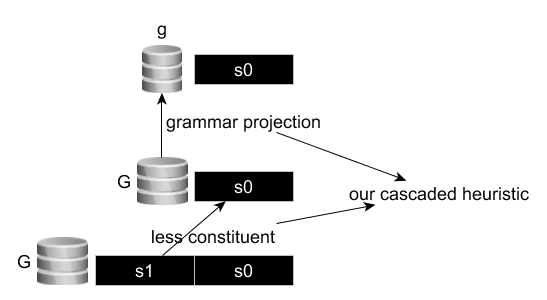
\includegraphics[width=0.5 \textwidth]{cascadedAstar.png}
	\caption{\label{spanFeature}The span feature from adapted from \cite{ref:2014David}.}
\end{figure}